% !TEX TS-program = pdflatexmk
\documentclass[11pt]{article}
\usepackage[margin=1in]{geometry} 
\usepackage[parfill]{parskip}% Begin paragraphs with an empty line rather than an indent 
\usepackage{graphicx} 
\usepackage{url}
%SetFonts
% newtxtext text and newtxmath
\usepackage{amsthm}
\newtheoremstyle{oldplain}
  {\topsep}   % ABOVESPACE
  {\topsep}   % BELOWSPACE
  {\itshape}  % BODYFONT
  {}       % INDENT (empty value is the same as 0pt)
  {\bfseries} % HEADFONT
  {.}         % HEADPUNCT
  {5pt plus 1pt minus 1pt} % HEADSPACE
  {}          % CUSTOM-HEAD-SPEC
\theoremstyle{oldplain}
\newtheorem{oldthm}{Theorem}[section]
\theoremstyle{plain}
\newtheorem{thm}{Theorem}[section]  
\pdfmapfile{=newtx.map}
\usepackage[osf,largesc,theoremfont]{newtxtext}
\usepackage[T1]{fontenc}
\usepackage[varqu,varl]{zi4}
\usepackage{amsmath}
\usepackage[bigdelims]{newtxmath}
%\useosf
\usepackage{bm}
%SetFonts
\usepackage{booktabs}
\title{New TX font package}
\author{Michael Sharpe}
\date{\today}  % Activate to display a given date or no date

\begin{document}
\maketitle
\section{Introduction}
This package is meant to be a replacement for Young Ryu's {\tt txfonts}. It is  a complete text ({\tt newtxtext}) and math ({\tt newtxmath}) package with roman text font provided by  a Times clone, sans serif based on a \textsf{Helvetica} clone, typewriter faces, plus math symbol fonts whose math italic letters are from a Times Italic clone. As of version 1.4, {\tt newtxtext} no longer depends on {\tt txfonts} but is based on the richer source \textsf{TeXGyre Termes}, but {\tt newtxmath} continues to use the {\tt txfonts} math glyphs with many metric adjustments and some wholesale modifications.

This math package works, after possibly replacing its math Roman and Greek letters, with fonts other than Times that are intermediate in weight between Computer Modern and Times. The free font Linux Libertine is one particular target---it is of nearly the same x-height as Computer Modern, but, not being a \emph{modern} font, does not have a high contrast ratio, and so appears  denser than Computer Modern but not as much so as Times. It is meant as a replacement for Times, but  differs from it in many characteristics, more similar to MinionPro than Times, and provides a better range of variants than Times---three weights (regular, semi-bold and bold) rather than just two, and has expert features in all weights: old-style figures, more extensive and more interesting ligatures,  and  small caps. In my opinion, material typeset in Linux Libertine looks better than the corresponding material typeset in Times. This seems especially true on the screen. As of version 1.0, the package also offers support for MinionPro as a math font, but with limitations described in detail below. More recently, an option to provide math support for the \textsf{garamondx} text font package was added.

The {\tt newtx} package differs from {\tt txfonts} in the following ways:
\begin{itemize}
\item
the new package is split into separate text and math packages that do not need to be used in conjunction;
\item both text and math packages offer options not present in the original package, described below, including the option to use \textsf{libertine} Latin and Greek letters to replace \textsf{Times}, as well as a similar option \textsf{minion};
\item wide accent glyphs have been corrected (they should have zero depth) so that they no longer collide with the underlying glyph;
\item for those who do not like the integral in \textsf{txfonts}, an emboldened version of the Computer Modern integral is made available, matching the weight of the \textsf{txfonts} symbols;
\item an upright partial derivative symbol has been added, named \verb|\uppartial|;
\item there is now an option to get braces more pleasing to older eyes;
\item macros have been added to bring the calls to Greek symbols more into conformity with \textsc{psnfss} and Mathtime Pro~2;
\item problems using \textsc{ams} macro packages before \textsf{txfonts} are settled;
\item \verb|\coloneq| and \verb|\eqcolon| now point to the correct glyphs;
\item The problem with the {\tt ogonek} accent  and tabular environments (bad definition of \verb|\k|) is fixed;
\item The default encoding for \textsf{newtxtext} is now T$1$, but support is offered also for OT$1$ and LY$1$. As some add-on packages are available only in T$1$, that seems the best current choice.
\item Sans serif is by default taken from TeXGyreHeros, and by default at 90\% of the scale factor (set by {\tt scaled}, default value {\tt1}). The option {\tt helvratio=.98} will change that to 98\%.
\item \verb|\varkappa| $\varkappa$ has been moved from {\tt AMSb} to {\tt lettersA}, and is now accompanied by an upright form \verb|\upvarkappa| $\upvarkappa$ which behaves as it should when using the {\tt frenchmath} option.
\end{itemize}
\section{Text mode options}
Beginning with version 1.4, the text font component of \textsf{newtx} is no longer dependent on the {\tt txfonts}, and is constructed entirely from \textsf{TeXGyre Termes} and some modifications thereof.

The text mode environment invoked by
\begin{verbatim}
\usepackage{newtxtext}
\end{verbatim}
has several options, a number new to version 1.4: you may write
\begin{verbatim}
\usepackage[scaled=.93]{newtxtext}
\end{verbatim}
to load the roman and typewriter text fonts at 93\% of normal size, and the sans serif (\textsf{Helvetica} clone) at scale $0.9*0.93$. This is not of much utility if the package is used with the math package {\tt newtxmath} to which it is already matched, but may be with other math packages. The options
\begin{verbatim}
\usepackage[scaled=.95,helvratio=.96]{newtxtext}
\end{verbatim}
load roman and typewriter text fonts at 95\% of normal size, and the sans serif (\textsf{Helvetica} clone) at scale $0.95*0.96$.

The option \texttt{osf} instructs the text fonts to use old-style figures \oldstylenums{1234567890} rather than the default lining figures $1234567890$. As of version $1.23$, {\tt newtxtext} loads initially with lining figures so the math package uses lining figures in math mode. The option {\tt osf} switches to old-style figures in text at the very end of the preamble, forcing the use of oldstyle figures in text, but not math. In previous versions, it was necessary to run 
\verb|\useosf| after loading math. This is no longer required, but does no harm. 

There is one special case where \verb|\useosf| is necessary: in you use the {\tt babel} package, you should load it before {\tt newtxtext}---for example:
%may receive puzzling error messages if you used a preamble containing
\begin{verbatim}
\usepackage[<babel options>]{babel}
\usepackage[osf]{newtxtext}
% works as expected if no math package loaded
\end{verbatim}
If you want to use {\tt babel} and a math package, you have to be aware of an incompatibility between some {\tt babel} code and the {\tt etoolbox} command \verb|\AtEndPreamble|. In this case, use instead the more cumbersome form:
\begin{verbatim}
\usepackage[<babel options>]{babel}
\usepackage{newtxtext}
<other babel font loading commands>
\usepackage{newtxmath}
\useosf % must be after loading math package
\end{verbatim}
As of version 1.4, there are four normal figure styles: tabular lining, tabular oldstyle, proportional lining and proportional oldstyle, the default figure alignment being \texttt{tabular}. To switch to \texttt{proportional}, use the option \texttt{p} or \texttt{proportional}.

Option {\tt defaultsups} (same effect as {\tt defaultsups=true}) forces the package to use the \LaTeX\ default footnote markers (or, at least, those in force when the package is loaded) instead of those preferred by the package---Times Roman superior figures instead of spindly ordinary Times lining figures reduced to about 70\%. (Footnote markers in minipages use the default lowercase italic alphabetic characters, unless otherwise specified by redefining \verb|\thempfootnote|.) For better control over position and size of footnote markers, use the {\tt superiors} package after loading {\tt newtxtext}. The \verb|\sustyle| font switch and its related \verb|\textsu| macro know not only about figures, but also the lower case letters, including \texttt{egrave}, so that traditional French expressions like \textlf{1}\textsu{i\`ere} may be typeset correctly.

Option \texttt{largesc} changes the small cap glyphs from the default petite caps defined in TeXGyre Termes (same size as in txfonts) to a larger size that, in upright shapes, is metrically compatible with Adobe's small caps. These are about 10\% larger than petite caps. For a comparison, \textsc{Small Caps}, {\usefont{T1}{qtm}{m}{sc}Petite Caps}, and \textsc{\textit{Italic Small Caps}}, {\usefont{T1}{qtm}{m}{scit}Italic Petite Caps}.

Option \texttt{adobesc} is only for those who own licenses for \textsf{Adobe Times Small Caps} and install them into the \texttt{ptmsc} package downloaded from \textsc{ctan}. This option loads \texttt{largesc} and substitutes the Adobe glyphs, where available, including their larger Regular and Bold tabular oldstyle figures.

The {\tt theoremfont} option changes the default font used for the {\tt plain} theoremstyle of {\tt amsthm}, keeping italic text but substituting upright figures and punctuation, and, provided you have loaded {\tt theorem} or {\tt amsthm} before {\tt newtxtext}, it will redefine the plain theoremstyle.  For example, with this option, you get theorem statements like this:

\begin{thm}
This is Theorem Italic: text numbers are upright---12345; punctuation is in many cases upright (also, parens, braces \{\} and brackets []). What about question marks and exclamations? Also upright! [These fit better with math mode punctuation and figures, like: for all $x\in[0,1]$, let $f(x)\coloneq \exp(\alpha x)$].
\end{thm}
Compare this to traditional {\tt plain} theoremstyle with the same text:
\begin{oldthm}
This is Theorem Italic: text numbers are upright---12345; punctuation is in many cases upright (also, parens, braces \{\} and brackets []). What about question marks and exclamations? Also upright! [These fit better with math mode punctuation and figures, like: for all $x\in[0,1]$, let $f(x)\coloneq \exp(\alpha x)$].
\end{oldthm}
\section{Math mode options}
The package invoked by
\begin{verbatim}
\usepackage{newtxmath}
\end{verbatim}
loads the math part of the {\tt txfonts} (with revised metrics and additional glyphs) and should be loaded \emph{after} the text font and its encoding have been specified, as it uses the text font settings to define how operators, numbers, math accents, \verb|\mathrm|, \verb|\mathbf| etc.\ are rendered. You should also load a Typewriter font so as not to generate mysterious error messages about \textsf{metafont} trying to generate \texttt{ectt10}. The package offers a number of options.
\begin{itemize}
\item {\tt varg} causes the math italic letters \verb|g,v,w,y| to be replaced by versions which are more distinctive---eg, useful for distinguishing math italic \verb|v| from \verb|\nu|;
\item {\tt libertine} loads different versions of math italic and bold math italic based on \textsf{Libertine} rather than \textsf{Times}---the {\tt varg} option is disabled in this case, as the equivalent variant forms are made available by default;
\item {\tt minion} loads different versions of math italic and bold math italic based on \textsf{MinionPro} rather than \textsf{Times}---the {\tt varg} option is disabled in this case, as the equivalent variant forms are made available by default---see the extended discussion below;
\item {\tt garamondx} loads different versions of math italic and bold math italic based on \textsf{garamondx} rather than \textsf{Times}---the {\tt varg} option is disabled in this case, as the equivalent variant forms are made available by default.
\item {\tt baskervaldx} (or {\tt Baskervaldx}) loads different versions of math italic and bold math italic based on \textsf{Baskervaldx} rather than \textsf{Times}---the {\tt varg} option is disabled in this case, as the equivalent variant forms are made available by default.
\item {\tt utopia} (or {\tt heuristica} or {\tt erewhon}) loads different versions of math italic and bold math italic based on \textsf{Utopia} rather than \textsf{Times}---the {\tt varg} option is disabled in this case, as the equivalent variant forms are made available by default. The Heuristica or Erewhon font package must be installed to use this option. (Erewhon is based on Heuristica, but is 6\% smaller and has more complete figures styles and small cap style, as well as a variety of smaller figures---superior, inferior, numerator, denominator.)  For example:
\begin{verbatim}
\usepackage[osf]{erewhon} %extension of Utopia
\usepackage[varqu,varl]{inconsolata} % sans typewriter
\usepackage[scaled=.95]{cabin} % sans serif
\usepackage[utopia,bigdelims,vvarbb]{newtxmath}
\end{verbatim}
\item the {\tt libertine} option also replaces both slanted and upright Greek  symbols by the corresponding Libertine glyphs, and similarly for {\tt minion} and {\tt garamondx};
\item
{\tt cmintegrals} instructs \textsf{newtxmath} to load a thicker version of the Computer Modern integral in place of the \textsf{newtxmath} default---the txfonts integral (identical to the integral in the Wolfram fonts), which is not to everyone's taste---a consequence is that none of the special forms of \textsf{txfonts} integrals are available;
\item the combination
\begin{verbatim}
\usepackage{amsmath}% loads amstext, amsbsy, amsopn but not amssymb
\usepackage{newtxmath}
\end{verbatim}
causes no error, unlike the same combination with {\tt txfonts}, but does nothing significant. (Recall that {\tt amsmath} is loaded automatically if you use an \textsc{ams} document class such as {\tt amsart} or {\tt amsbook}, as is {\tt amsthm}.) The integrals are as defined in {\tt txfonts}. On the other hand,
\begin{verbatim}
\usepackage{amsmath}
\usepackage[cmintegrals]{newtxmath}
\end{verbatim}
allows you to use the forms \verb|\iint|, \verb|\iiint|, \verb|\iiiint| and \verb|\idotsint| defined in {\tt amsmath}, but using the pumped-up Computer Modern integral loaded by {\tt newtxmath}. 
\item {\tt uprightGreek} and {\tt slantedGreek} determine the form of Greek alphabet loaded---the default is {\tt uprightGreek}, which loads upright uppercase and slanted lowercase Greek symbols, as is customary in Anglo-American mathematical typesetting. With the option {\tt slantedGreek}, which you might want to use if you cared about ISO standards, all Greek symbols are slanted. No matter which is set, \verb|\Gammaup| (or \verb|\upGamma|) gives you upright \verb|\Gamma|, etc.
\item Option {\tt frenchmath} sets the default style in math mode for rendering uppercase Roman and Greek letters to upright, and lowercase Greek letters to upright. (Introduced in v.\ 1.28.)
\item The option {\tt cmbraces} instructs {\tt newtxmath} to ignore the brace collections from {\tt txfonts}, substituting a collection based on thickened versions of the Computer Modern braces, which I find much easier to distinguish from other delimiters. This works quite well in regular weight but looks a bit clunky in bold. I now prefer the option {\tt bigdelims}, which supersedes {\tt cmbraces}.
\item The \textsf{newtxmath} package contains three different Blackboard Bold alphabets, where original \textsf{txfonts} contained two. The default, triggered by \verb|\mathbb{}|, takes its glyphs from the font which replaces {\tt msbm} and has the same overall appearance of a hollowed-out text font, which I find neither bold nor blackboard-like. The second option, taken from \textsf{txfonts}, is triggered by \verb|\varmathbb{}|, is more geometric and, in my opinion, preferable but not optimal. The option {\tt varbb} makes \verb|\mathbb{}| synonymous with \verb|\varmathbb{}|. The third option is the double-struck glyphs from the STIX collection. See the expanded discussion below.
\item {\tt nosymbolsc} causes the package to not load the {\tt symbolsC} fonts, saving  a math family. (This font contains mostly exotic symbols, along with some very useful, commonly used symbols like \verb|\coloneq| $\coloneq$, \verb|\eqcolon| $\eqcolon$, \verb|\notin| $\notin$, \verb|\notni| $\notni$, \verb|\neq| $\neq$, \verb|\nsubset| $\nsubset$ and \verb|\nsupset| $\nsupset$, but these have been moved (virtually) to {\tt lettersA} so they may continue to be used even if you use the option {\tt nosymbolsc}.)
\item {\tt amssymbols} (the default) and {\tt noamssymbols} determine whether the {\tt txfonts} versions of the \textsc{ams} symbols ({\tt msam}, {\tt msbm}) are loaded---if so, they override previous settings in {\tt amsmath}. If you use the option {\tt noamssymbols}, then \verb|\mathbb{}| is set to mean the same as \verb|\varmathbb{}|. (One advantage of {\tt noamssymbols} is that you save two of your precious math families for other purposes, such as setting a couple of external math alphabets by means of the \textsf{mathalfa} package.)
\item {\tt libaltvw} has effect only if the libertine option is selected---in this case, it substitutes for math italic v and w hand-crafted versions based on the Libertine upsilon glyphs.
\item{\tt bigdelims} loads a different math extension font and redefines most of the small and big math delimiters to have larger sizes so that, for example, there is more of a distinction between \verb|(| and \verb|\big(| in math mode. If this option is specified, {\tt cmbraces} is ignored.
\item{\tt liby} has an effect only if the libertine option is selected---with this option, the math italic y is chosen to be Libertine's italic y instead of the default one from txfonts.
\item As of version $1.18$ of {\tt newtxmath} (and version $1.07$ of {\tt newpxmath}) there are new math accents and macros available.
\begin{itemize}
\item
\verb|\widehat| and \verb|\widetilde| have been extended from $3$ to $6$ sizes, and the smallest is now not as wide as in previous versions. In particular, you can now use, eg, \verb|$\widehat{X}^2$|, which gives $\widehat{X}^2$ without the hat colliding with the superscript.
\item The math double bracket delimiters have been moved to another family so their use is less likely to cause a ``too many math families'' error. The ordinary sizes now have their own macros, \verb|\dlb| and \verb|\drb|, giving, eg, $\dlb 0,T\drb$, as commonly used in probability theory.
\item The new macros \verb|\overgroup|, \verb|\undergroup|, \verb|\overgroupra|, \verb|\overgroupla|, \verb|\undergroupra| and \verb|\undergroupla| are intended as replacements for the \verb|\wideparen| and related macros from the \textsf{yhmath} and \textsf{fourier} packages. In fact, \verb|\overgroup| and \verb|\undergroup| are variants of the existing macros \verb|\overbrace| and \verb|\underbrace|, while the suffixes {\tt ra} and {\tt la} signify right arrow and left arrow respectively. The macro \verb|\widering| places a ring centered over an \verb|\overgroup|, not dissimilar from its use in {\tt yhmath}. Example:
\begin{verbatim}
\[\overgroup{ABC}\quad\overgroupra{ABC}\quad\undergroup{ABC}\quad
\undergroupla{ABC}\quad \widering{ABCD}\] 
\end{verbatim}
gives
\[\overgroup{ABC}\quad\overgroupra{ABC}\quad\undergroup{ABC}\quad\undergroupla{ABC}\quad\widering{ABCD}\] 
\end{itemize}
\item As of version $1.23$, the package contains new math accents \verb|\widearc| and \verb|\wideOarc| similar in effect to those from \textsf{fourier} and \textsf{kpfonts}. Example: 
\begin{verbatim}
\[\widearc{BC}\quad\widearc{ABC}\quad\widearc{ABCD}\quad
\wideOarc{BC}\quad\wideOarc{ABC}\quad\wideOarc{ABCD}\]
\end{verbatim}
gives
\[\widearc{BC}\quad\widearc{ABC}\quad\widearc{ABCD}\quad
\wideOarc{BC}\quad\wideOarc{ABC}\quad\wideOarc{ABCD}\]
%\item {largelibfigs} has effect only if the libertine option is selected---with this option, full-sized figures are substituted in math mode for the default Libertine figures, which are about 8\% below Libertine's Capheight.
\item The option {\tt timesmathacc} changes the default selection of math accents from the Roman text font, forcing the use of the heavier Times accents. (Libertine has much lighter accents which can seem to almost disappear under some conditions.) If your language uses accented operator names, do not use this option.
\end{itemize}
\bigskip

\textbf{IMPORTANT:} The Libertine text package is now once again named {\tt libertine}, but requires arguments that are different from the original {\tt libertine} package.

\textsc{Example 1:}
\begin{verbatim}
\usepackage[osf]{newtxtext} % T1, lining figures in math, osf in text
\usepackage{textcomp} % required for special glyphs
\usepackage{amsmath}
\usepackage[varg,cmintegrals,bigdelims]{newtxmath}
\usepackage{bm} % load after all math to give access to bold math
%\useosf %no longer required if osf specified
\end{verbatim}
\textsc{Example 2:}
\begin{verbatim}
\usepackage[lining,semibold]{libertine} % a bit lighter than Times--no osf in math
\usepackage[T1]{fontenc} % best for Western European languages
\usepackage{textcomp} % required to get special symbols
\usepackage[varqu,varl]{inconsolata}% a typewriter font must be defined
\usepackage{amsmath,amsthm}
\usepackage[libertine,cmintegrals,bigdelims,vvarbb]{newtxmath}
\usepackage[scr=rsfso]{mathalfa}
\usepackage{bm}% load after all math to give access to bold math
%After loading math package, switch to osf in text.
\useosf % for osf in normal text
\end{verbatim}

\textbf{Caution:} In encodings {\tt T1} and {\tt LY1}, the macro \verb|\mathrm| does not produce what you might expect for Greek letters, due to the difference between those encodings and {\tt OT1}. But what were you expecting with \verb|\mathrm{Gamma}| anyway? In {\tt T1} and {\tt LY1}, you'll get a math accent.

\section{Usage with Lua\LaTeX\ and Xe\LaTeX}
As far as I can tell, \textsf{newtxmath} works with both, but requires a very specific loading order and choice of options. Briefly, except for {\tt libertine} text, the math options must all be loaded prior to loading and using {\tt fontspec}. Be aware that some text packages (eg, {\tt cabin}) may contain a line like
\begin{verbatim}
\RequirePackage{fontspec}
\end{verbatim}
which would prevent (``option clash'' error) a subsequent 
\begin{verbatim}
\usepackage[no-math]{fontspec}
\end{verbatim}
unless suppressed by an appropriate option. Eg, 
\begin{verbatim}
\usepackage[type1]{cabin}
\end{verbatim}
prevents the problem with the {\tt cabin} package.

The following examples illustrate some general models, the most unintuitive being the first because it loads a small version, {\tt minlibertine}, of libertine text for use in math mode as numbers, basic symbols and operators.

\textsc{Example 3:}
\begin{verbatim}
%load text components other than libertine text to be used in math
\usepackage[T1]{fontenc}
\usepackage[scaled=.85]{beramono}% used only by \mathtt
\usepackage[type1]{cabin}% used only by \mathsf
\usepackage{amsmath,amsthm}
\usepackage[libertine,bigdelims]{newtxmath}
% loads minlibertine because no other Roman text package was specified
% so that \mathrm and \mathbf also use minlibertine
\usepackage[scr=rsfso]{mathalfa}
\usepackage{bm}% load after all math to give access to bold math
%Now load the otf text fonts using fontspec---won't affect math
\usepackage[no-math]{fontspec} % process with XeLaTeX or LuaLaTeX
\usepackage{libertine}
%\usepackage[osf,semibold]{libertine} for osf in text, semibold as bold
\end{verbatim}
The next example is similar, but in math mode, numbers, basic symbols, operator names, \verb|\mathrm| and \verb|\mathbf| will render with {\tt fbb-LF}, though  math italic and math Greek letters will be from {\tt libertine}. (Note that one specifies the encoding and redefines \verb|\rmdefault|. For reasons I don't yet understand, it may not work to load the font package---ie, don't substitute \verb|\usepackage{fbb}|, as that will mess up bold in the libertine text package.) 

\textsc{Example 4:}
\begin{verbatim}
%load text components other than libertine text to be used in math
\usepackage[T1]{fontenc}
\renewcommand{\rmdefault}{fbb-LF}% Roman font for use in math mode
\usepackage[scaled=.85]{beramono}% used only by \mathtt
\usepackage[type1]{cabin}% used only by \mathsf
\usepackage{amsmath,amsthm}
\usepackage[libertine,cmintegrals,bigdelims,vvarbb]{newtxmath}
% does not load minlibertine because another Roman text package was specified
\usepackage[scr=rsfso]{mathalfa}
\usepackage{bm}% load after all math to give access to bold math
%Now load the otf text fonts using fontspec---won't affect math
\usepackage[no-math]{fontspec} % process with XeLaTeX or LuaLaTeX
\usepackage{libertine}
\end{verbatim}


\section{Alternate forms of glyphs}
Several math glyphs have alternate forms:
\begin{center}
  \begin{tabular}{@{} llll @{}}
    \hline
    Command & Result &  Alternate Commands & Alternate Forms\\ 
    \hline
    \verb|\emptyset| & $\emptyset$ & \verb|\varnothing, \emptysetAlt|& $\varnothing, \emptysetAlt$ \\ 
    \verb|\forall| & $\forall$ & \verb|\forallAlt| & $\forallAlt$ \\ 
    \verb|\exists| & $\exists$ & \verb|\existsAlt| & $\existsAlt$ \\ 
    \verb|\nexists| & $\nexists$ & \verb|\nexistsAlt| & $\nexistsAlt$ \\ 
    \hline
  \end{tabular}
\end{center}
You should be aware that using \verb|\varnothing| requires loading AMSb.\\
To use an alternate form throughout your document without changing all occurrences of the usual command, insert something like the following in your preamble after loading \texttt{newtxmath}:
\begin{verbatim}
\let\forall\forallAlt
\end{verbatim}
\section{Conformity with amsmath}
The {\tt newtxmath} package now contains a \verb|\RequirePackage{amsmath}|, as it uses a number of the macros defined there. To pass options to {\tt amsmath}, you can pass the options as options to \verb|\documentclass|. For example,
\begin{verbatim}
\documentclass[11pt,intlimits]{article}
\usepackage{newtxtext}
\usepackage[bigdelims]{newtxmath}
\end{verbatim}
will load {\tt amsmath} with option {\tt intlimits}. As of version 1.14, {\tt newtxmath} respects the {\tt amsmath} macros for placement of limits on integrals.

\section{The {\tt minion} option}
This option allows the use of MinionPro as math letters (Latin and Greek) within  the math font, but there are some caveats:
\begin{itemize}
\item
you must use a recent version of MinionPro, such as the version that comes with recent versions of Adobe Reader. In addition, the fonts must installed under special names so they can be recognized by the support files---this is spelled out in the documentation for the minion2newtx package that must be downloaded from \url{CTAN.tug.org} and installed separately.
\end{itemize}

\section{The \TeX\ math font problem}
Math font packages in \LaTeX\ are susceptible to the ``Too many math alphabets'' error, due to exceeding the limit of just sixteen math font families, or mathgroups, as they are called in \LaTeX. Put in oversimplified terms that do however correctly represent how this all works in \textsf{newtxmath}, the following math fonts are always loaded and permanently (if you didn't prevent loading of some features) occupying slots immediately following \verb|\begin{document}|, and others that may be called for in typesetting a mathematical expression can add to the list as the document grows.

\textsc{Always loaded:}
\begin{verbatim}
0: operators
1: letters
2: symbols
3: largesymbols
4: AMSa
5: AMSb
6: lettersA
7: symbolsC
8: largesymbolsTXA
9: boldoperators
10: boldletters
11: boldsymbols
12: boldlargesymbols
\end{verbatim}
\textsc{Notes:}
\begin{itemize}
\item
The {\tt operators} font is essentially the Roman text font, used for names of operators and as the target for \verb|\mathrm|---its bold version is used as the target for \verb|\mathbf|;
\item if you typeset an expression that, say, calls for a single bold glyph from  {\tt symbolsC}, that costs you an entire new slot, leaving only two remaining;
\item same with, eg, \verb|\mathit|;
\item same with an external Fraktur, Blackboard Bold or Script glyphs;
\item if you run out of math alphabets, look first to dropping {\tt AMSa} and {\tt AMSb}, as well as {\tt symbolsC}, which can save you three slots;
\item if space is tight, do not call bold versions of the fonts listed above where the bold version is not already loaded, to avoid loading a new mathgroup; 
\item if you absolutely need a letter (not a math symbol) from some math font that would normally cost you another mathgroup, you might consider using as if it were text, with something like
\begin{verbatim}
\mbox{{\usefont{U}{ntxmia}{b}{n} X}}
\end{verbatim}
which allows you to use letter X from {\tt boldlettersA} but without any math features;
\item there is a macro \verb|\ShowMathFonts| in {\tt newtxmath} which may be called at any point in your document, which will provide you a list of the mathgroups currently in use. This can be helpful in figuring out where problems occur. The output lines take the form
\begin{verbatim}
(<fam number>: <internal font id> = <tfm name> [newtx name])
\end{verbatim}

\end{itemize}
\section{Bold math fonts}\label{sec:boldmath}
Every math font in the {\tt txfonts} package, and in the {\tt newtx} package, is accompanied by a bold version. Some usage examples are given below. Generally, one may use either \verb|\boldmath| to change an entire formula to bold, or \verb|\boldsymbol| to change one symbol, but the spacing generally works better after loading the {\tt bm} package and using the \verb|\bm| macro.

The text glyphs dotlessi (\verb|\i|) and dotlessj (\verb|\j|) are rarely needed in actual text---in many fonts, roman dotlessi is very similar to the numeral 1. They are however sometimes needed to build special math glyphs. The following table shows how to generate the mathematical forms of dotlessi and dotlessj. I illustrate with only dotlessi---dotlessj is entirely analogous.

\begin{center}
  \begin{tabular}{@{} llll @{}}
    \hline
    Type & Weight & Command & Result \\ 
    \hline
    Math Italic & Regular & \verb|$\hat{\imath}$| & $\hat{\imath}$ \\ 
    Math Italic & Bold & \verb|$\bm{\hat{\imath}}$| & $\bm{\hat{\imath}}$ \\ 
    Roman & Regular & \verb|$\hat{\textrm{\i}}$| & $\hat{\textrm{\i}}$\\ 
    Roman & Bold & \verb|$\bm{\hat{\textbf{\i}}}$| & $\bm{\hat{\textbf{\i}}}$\\ 
    \hline
  \end{tabular}
\end{center}
\newcommand{\xyvec}[2]{\ensuremath{#1\mkern1.5mu\bm{\textbf{\i}}#2\mkern1.5mu\bm{\textbf{\j}}}}

In math, bold roman characters are often used to indicate vector quantities, and for this one uses constructions like 
\begin{itemize}
\item
\verb|$\mathbf{x}$| produces $\mathbf{x}$;
\item
\verb|$\bm{\mathrm{x}}$| produces $\bm{\mathrm{x}}$ (same as previous but may offer improved spacing);
\item
\verb|$\bm{x}$| produces $\bm{x}$ (not roman);
\item
\verb|$\bm{\hat{\mathbf{x}}}$| produces $\bm{\hat{\mathbf{x}}}$ (with a bold accent);
\item \verb|$\bm{\dot{x}}$| produces $\bm{\dot{x}}$ (bold but not roman);
\item the macro definition
\begin{verbatim}
\newcommand{\xyvec}[2]{%
\ensuremath{#1\mkern1.5mu\bm{\textbf{\i}}#2\mkern1.5mu\bm{\textbf{\j}}}}
\end{verbatim}
allows you to write \verb|\xyvec{x}{+y}| to output $\xyvec{x}{+y}$;
\item \verb|$\bm{\Gamma}$| produces $\bm{\Gamma}$ (bold Gamma);
\item \verb|$\bm{\hat{\Gamma}}$| produces $\bm{\hat{\Gamma}}$ (bold Gamma with bold accent).
\end{itemize}
(The last two assume that you have effectively set the option {\tt uprightGreek}---the default.)

\section{Blackboard bold}
As mentioned briefly above, the package now has a new blackboard bold alphabet built-in, and some new macros to call the non-default versions. To summarize, the problems are:
\begin{itemize}
\item
the default, called by \verb|\mathbb| is quite ugly and indistinct, but does cooperate with the bolding macros \verb|\bm| and \verb|\boldsymbol|;
\item the original variant form called with the macro \verb|\varmathbb| is better, but the macro conflicts with \verb|\bm|. (In fact, the bold version is identical to the regular version, but it is still not right that it conflicts with them.) The problem stems from the part of the definition of \verb|\varmathbb| which allows you to insert an argument with more than one character, like \verb|\varmathbb{ABC}|. Another problem with \verb|\varmathbb| is that it conflicts with {\tt hyperref}---if you use the macro in a moveable argument such as a section heading, you will provoke a \LaTeX\ error message. The solution is to use macros that take a single character as argument, like \verb|\vmathbb{A}| and \verb|\vvmathbb{A}|, which both cooperate with \verb|\bm| and {\tt hyperref}.
\item the third, new, alphabet is borrowed from the STIX fonts---it is sharp and quite clear, geometric in design. The only slight problem is that it lacks a full bold version, with only the letters C, D, H, N, P, Q, R, Z, d, e, i and j available. The macro \verb|\vvmathbb| provided to access this alphabet allows only a single character for its argument. The new option {\tt vvarbb} effectively makes \verb|\mathbb| mean the same as \verb|\vvmathbb|.
(The reason for including these in the \textsf{newtx} package rather than calling them from the \textsf{mathalfa} package is that \textsf{newtx} leaves very little space for new math symbol fonts and math alphabets, and this way requires no additional such resources.
\end{itemize}
One interesting feature of the new alphabet is that it contains blackboard bold numbers, of which $0$ and $1$ will likely be the most useful, perhaps as operator names. I find $\vvmathbb{1}$=\verb|$\vvmathbb{1}$| useful in specifying an indicator, AKA characteristic function. Here are some examples:

\begin{center}
  \begin{tabular}{@{} llll @{}}
    \toprule
     & Regular & Bold & Remarks \\ 
    \midrule
Default  & \verb|$\mathbb{R}$| $\mathbb{R}$& \verb|$\bm{\mathbb{R}}$| $\bm{\mathbb{R}}$\\ 
Variant 1     & \verb|$\varmathbb{R}$| $\varmathbb{R}$ &  & Bold is same as regular \\ 
$\dots$or     & \verb|$\vmathbb{R}$| $\vmathbb{R}$ &  & Single char.\ argument\\ 
Variant 2 & \verb|$\vvmathbb{R}}$| $\vvmathbb{R}$& \verb|{\boldmath $\vvmathbb{R}$}| {\boldmath $\vvmathbb{R}$} & Make a macro for this! \\ 
%     & $\bm{\mathbb{AB}}$  & $\bm{\vmathbb{A}\vmathbb{B}}$ & $\bm{\vvmathbb{A}\vvmathbb{B}}$ \\ 
    \bottomrule
  \end{tabular}
\end{center}

\section{Samples from free Times and Libertine packages}
\textsc{TXFONTS:}\\
\begin{verbatim}
\usepackage{txfonts}
\end{verbatim}
\[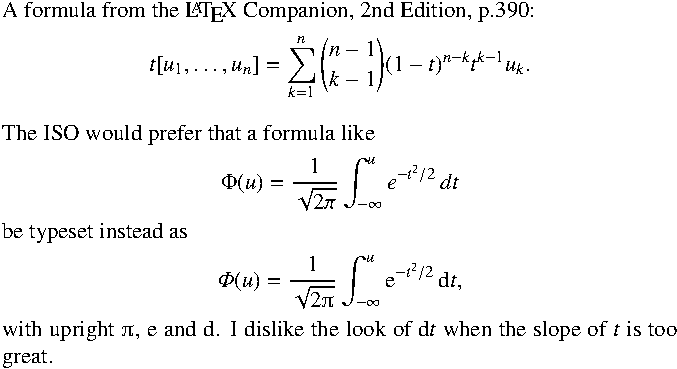
\includegraphics{sample-tx-crop}\]
\begin{itemize}
\item
Complete match between text and math size and weight;
\item first formula much too cramped;
\item upper limit of integral much too close to integral sign;
\item square on $t$ in integrand comes very close to colliding with it;
\item square root in denominator aligned too far right.
\end{itemize}

\vspace{1pc}
\textsc{NEWTXFONTS:}\\
\begin{verbatim}
\usepackage{newtxtext}
\usepackage{newtxmath}
\end{verbatim}
\[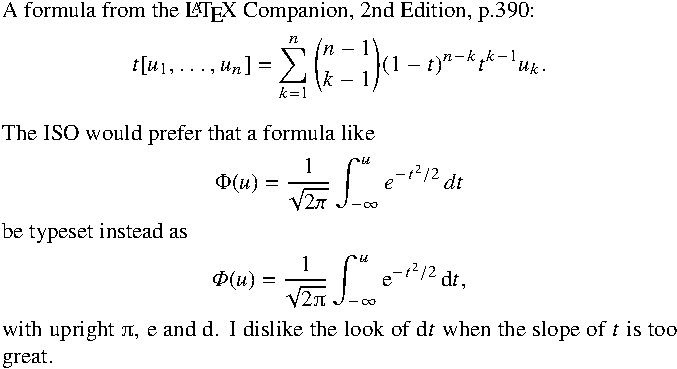
\includegraphics{sample-ntx-crop}\]
\begin{itemize}
\item
Complete match between text and math size and weight;
\item first formula much less cramped;
\item upper limit of integral not too close to integral sign;
\item square not too close to $t$ in exponent;
\item better alignment of square root in denominator.
\end{itemize}

\vspace{1pc}
\textsc{MathTimePro2:}\\
\begin{verbatim}
\usepackage{newtxtext}
\usepackage[lite]{mtpro2}
\end{verbatim}
\[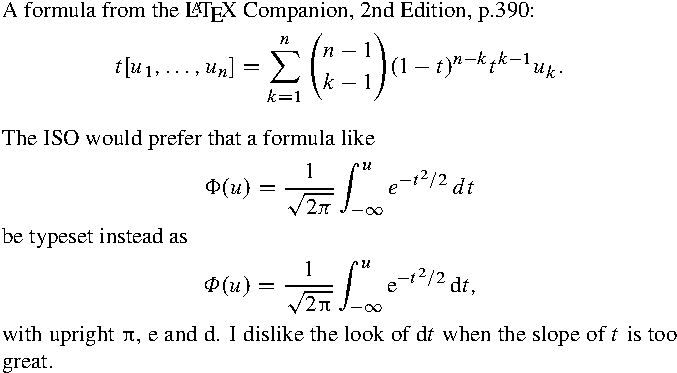
\includegraphics{sample-mtp-crop}\]
\begin{itemize}
\item
Complete match between text and math size and weight;
\item first formula quite spread out;
\item upper limit of integral not too close to integral sign;
\item plenty of space between square and $t$ in exponent.
\end{itemize}

\vspace{1pc}
\textsc{Libertine and MathTimePro2:}\\
\begin{verbatim}
\usepackage{libertine}
\usepackage[T1]{fontenc}
\usepackage[lite]{mtpro2}
\end{verbatim}
\[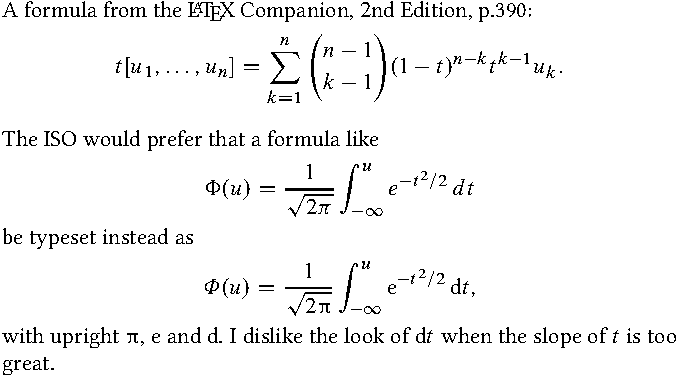
\includegraphics{sample-libmtp-crop}\]
\begin{itemize}
\item
Mismatch of weight between text and math;
\item first formula quite spread out;
\item upper limit of integral not too close to integral sign;
\item plenty of space between square and $t$ in exponent.
\end{itemize}

\vspace{1pc}
\textsc{Libertine and newtxmath:}\\
\begin{verbatim}
\usepackage{libertine}
\usepackage[T1]{fontenc}
\usepackage[libertine]{newtxmath}
\end{verbatim}
\[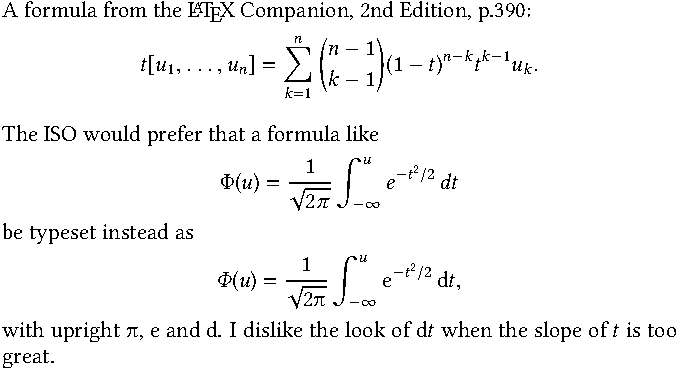
\includegraphics{sample-lib-crop}\]
\begin{itemize}
\item
Very good match between text and math in size and weight;
\item first formula not cramped;
\item upper limit of integral not too close to integral sign;
\item space between square and $t$ in exponent;
\item better alignment of square root in denominator.
\end{itemize}

\vspace{1pc}
\textsc{Mathptmx:}\\
\begin{verbatim}
\usepackage{mathptmx}
\end{verbatim}
\[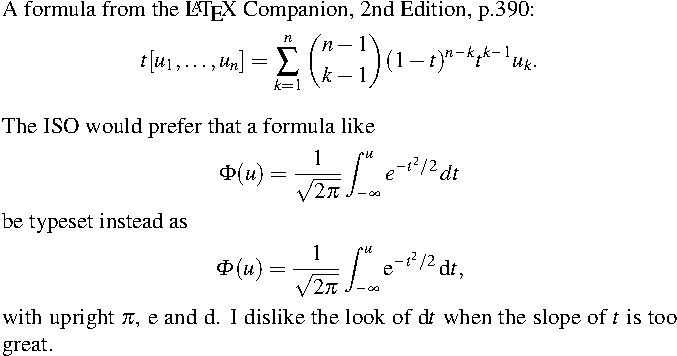
\includegraphics{sample-ptmx-crop}\]
\begin{itemize}
\item
Good match between text and math size and weight, though the summation symbol (from the system {\tt symbol} font) is too small and too dark;
\item first formula well spread;
\item upper limit of integral not too close to integral sign;
\item space between square and $t$ in exponent;
\item there are no upright Greek lowercase letters in this package;
\item good alignment of square root in denominator;
\item infinity symbol not sufficiently large?
\item the package lacks a number of amenities that are present in other packages.
\end{itemize}
\section{Items installed} As well as a collection of PostScript fonts, virtual fonts, font definition files and the central {\tt newtxtext.sty} and {\tt newtxmath.sty} files, the package contains one map file {\tt newtx.map} that must be enabled for the package to function correctly. Its name was changed from {\tt ntx.map} to mirror the package name.) The file \texttt{implementation.pdf} in this distribution provides a manifest of all files installed together with a brief indication of the sources. (This file is somewhat outdated. The file {\tt mathnotes.pdf} adds details about the sources for the math fonts, though it is rather cursory.)

The font files {\tt ntxexmods.pfb} and {\tt ntxbexmods.pfb} were derived from {\tt cmex10.pfb} by FontForgery, thickening the Computer Modern braces to match the weight of the \textsf{txfonts} braces. The pair {\tt ntxexb.pfb} and {\tt ntxbexb.pfb} were similarly derived from {\tt cmsy7.pfb} and {\tt cmex10.pfb} to produce more braces and matching integral signs based on Computer Modern. The {\tt.tfm} files {\tt rtx[b]mio.tfm} are simply unslanted versions of {\tt rtxmi}, from which we construct upright partial derivative symbols.
The last two entries provide us with a way to access custom-encoded versions of {\tt fxlri.pfb} and {\tt fxlbi.map} in order to access some of the unencoded alternate characters---eg, Greek letters, {\tt J.alt} and {\tt v.alt}. The font file \textsf{LibertineTheta-Regular.pfb} was created from the Theta symbol in {\tt fxlri.pfb}, which requires some FontForge help to look correct.

This version contains optical versions of the math italic and symbol fonts at 7\texttt{pt} and 5\texttt{pt}, allowing better rendering in \verb|\scriptstyle| and \verb|\scriptscriptstyle|. 

\end{document}  